\chapter{Putovi i ciklusi}

Ovo poglavlje bavi se dvjema vrstama putova u grafovima:
\begin{itemize}
\item \key{Eulerov put} je put koji
prolazi svakim bridom točno jednom.
\item \key{Hamiltonov put} je put
koji posjećuje svaki čvor točno jednom.
\end{itemize}

Iako Eulerovi i Hamiltonovi putovi na prvi pogled izgledaju
kao slični pojmovi,
računalni problemi vezani uz njih
vrlo su različiti.
Pokazuje se da postoji jednostavno pravilo koje
određuje sadrži li graf Eulerov put,
a postoji i efikasan algoritam za
pronalazak takvog puta ako on postoji.
Nasuprot tome, provjera postojanja Hamiltonovog puta je NP-težak
problem i nije poznat nijedan efikasan algoritam za njegovo rješavanje.

\section{Eulerovi putovi}

\index{Eulerov put}

\key{Eulerov put}\footnote{L. Euler proučavao je takve putove 1736. godine
kada je riješio poznati problem königsberških mostova.
To je bilo rođenje teorije grafova.} je put
koji prolazi točno jednom svakim bridom grafa.
Na primjer, graf
\begin{center}
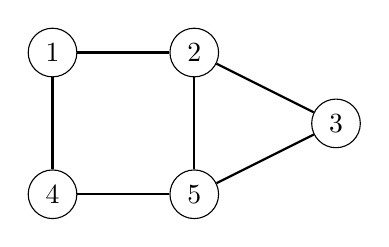
\begin{tikzpicture}[scale=0.9]
\node[draw, circle] (1) at (1,5) {$1$};
\node[draw, circle] (2) at (3,5) {$2$};
\node[draw, circle] (3) at (5,4) {$3$};
\node[draw, circle] (4) at (1,3) {$4$};
\node[draw, circle] (5) at (3,3) {$5$};

\path[draw,thick,-] (1) -- (2);
\path[draw,thick,-] (2) -- (3);
\path[draw,thick,-] (1) -- (4);
\path[draw,thick,-] (3) -- (5);
\path[draw,thick,-] (2) -- (5);
\path[draw,thick,-] (4) -- (5);
\end{tikzpicture}
\end{center}
ima Eulerov put od čvora 2 do čvora 5:
\begin{center}
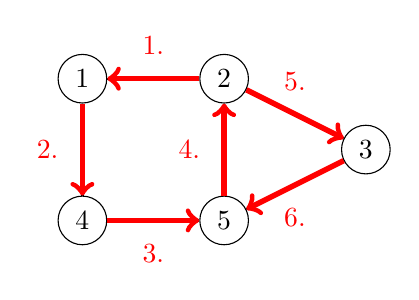
\begin{tikzpicture}[scale=0.9]
\node[draw, circle] (1) at (1,5) {$1$};
\node[draw, circle] (2) at (3,5) {$2$};
\node[draw, circle] (3) at (5,4) {$3$};
\node[draw, circle] (4) at (1,3) {$4$};
\node[draw, circle] (5) at (3,3) {$5$};

\path[draw,thick,-] (1) -- (2);
\path[draw,thick,-] (2) -- (3);
\path[draw,thick,-] (1) -- (4);
\path[draw,thick,-] (3) -- (5);
\path[draw,thick,-] (2) -- (5);
\path[draw,thick,-] (4) -- (5);

\path[draw=red,thick,->,line width=2pt] (2) -- node[font=\small,label={[red]north:1.}] {} (1);
\path[draw=red,thick,->,line width=2pt] (1) -- node[font=\small,label={[red]left:2.}] {} (4);
\path[draw=red,thick,->,line width=2pt] (4) -- node[font=\small,label={[red]south:3.}] {} (5);
\path[draw=red,thick,->,line width=2pt] (5) -- node[font=\small,label={[red]left:4.}] {} (2);
\path[draw=red,thick,->,line width=2pt] (2) -- node[font=\small,label={[red]north:5.}] {} (3);
\path[draw=red,thick,->,line width=2pt] (3) -- node[font=\small,label={[red]south:6.}] {} (5);
\end{tikzpicture}
\end{center}
\index{Eulerov ciklus}
\key{Eulerov ciklus}
je Eulerov put koji počinje i završava
u istom čvoru.
Na primjer, graf
\begin{center}
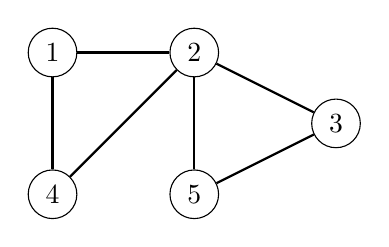
\begin{tikzpicture}[scale=0.9]
\node[draw, circle] (1) at (1,5) {$1$};
\node[draw, circle] (2) at (3,5) {$2$};
\node[draw, circle] (3) at (5,4) {$3$};
\node[draw, circle] (4) at (1,3) {$4$};
\node[draw, circle] (5) at (3,3) {$5$};

\path[draw,thick,-] (1) -- (2);
\path[draw,thick,-] (2) -- (3);
\path[draw,thick,-] (1) -- (4);
\path[draw,thick,-] (3) -- (5);
\path[draw,thick,-] (2) -- (5);
\path[draw,thick,-] (2) -- (4);
\end{tikzpicture}
\end{center}
ima Eulerov ciklus koji počinje i završava u čvoru 1:
\begin{center}
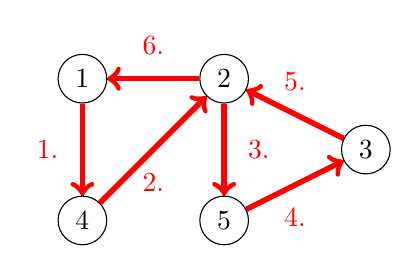
\begin{tikzpicture}[scale=0.9]
\node[draw, circle] (1) at (1,5) {$1$};
\node[draw, circle] (2) at (3,5) {$2$};
\node[draw, circle] (3) at (5,4) {$3$};
\node[draw, circle] (4) at (1,3) {$4$};
\node[draw, circle] (5) at (3,3) {$5$};

\path[draw,thick,-] (1) -- (2);
\path[draw,thick,-] (2) -- (3);
\path[draw,thick,-] (1) -- (4);
\path[draw,thick,-] (3) -- (5);
\path[draw,thick,-] (2) -- (5);
\path[draw,thick,-] (2) -- (4);

\path[draw=red,thick,->,line width=2pt] (1) -- node[font=\small,label={[red]left:1.}] {} (4);
\path[draw=red,thick,->,line width=2pt] (4) -- node[font=\small,label={[red]south:2.}] {} (2);
\path[draw=red,thick,->,line width=2pt] (2) -- node[font=\small,label={[red]right:3.}] {} (5);
\path[draw=red,thick,->,line width=2pt] (5) -- node[font=\small,label={[red]south:4.}] {} (3);
\path[draw=red,thick,->,line width=2pt] (3) -- node[font=\small,label={[red]north:5.}] {} (2);
\path[draw=red,thick,->,line width=2pt] (2) -- node[font=\small,label={[red]north:6.}] {} (1);
\end{tikzpicture}
\end{center}

\subsubsection{Postojanje}

Postojanje Eulerovih putova i ciklusa
ovisi o stupnjevima čvorova.
Prvo, neusmjereni graf ima Eulerov put 
točno onda kada svi bridovi
pripadaju istoj komponenti povezanosti i
\begin{itemize}
\item stupanj svakog čvora je paran \emph{ili}
\item stupanj točno dvaju čvorova je neparan,
a stupanj svih ostalih čvorova je paran.
\end{itemize}

U prvom slučaju svaki Eulerov put ujedno je i Eulerov ciklus.
U drugom slučaju čvorovi neparnog stupnja su početni
i završni čvor Eulerovog puta koji nije Eulerov ciklus.

\begin{samepage}
Na primjer, u grafu
\begin{center}
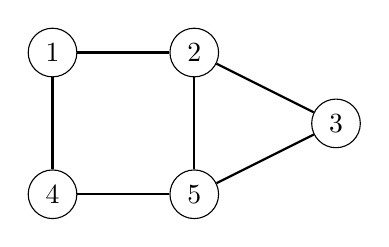
\begin{tikzpicture}[scale=0.9]
\node[draw, circle] (1) at (1,5) {$1$};
\node[draw, circle] (2) at (3,5) {$2$};
\node[draw, circle] (3) at (5,4) {$3$};
\node[draw, circle] (4) at (1,3) {$4$};
\node[draw, circle] (5) at (3,3) {$5$};

\path[draw,thick,-] (1) -- (2);
\path[draw,thick,-] (2) -- (3);
\path[draw,thick,-] (1) -- (4);
\path[draw,thick,-] (3) -- (5);
\path[draw,thick,-] (2) -- (5);
\path[draw,thick,-] (4) -- (5);
\end{tikzpicture}
\end{center}
\end{samepage}
čvorovi 1, 3 i 4 imaju stupanj 2,
a čvorovi 2 i 5 imaju stupanj 3.
Točno dva čvora imaju neparan stupanj,
pa postoji Eulerov put između čvorova 2 i 5,
ali graf ne sadrži Eulerov ciklus.

U usmjerenom grafu
promatramo ulazne i izlazne stupnjeve
čvorova.
Usmjereni graf sadrži Eulerov put
točno onda kada svi bridovi pripadaju istoj
komponenti povezanosti i
\begin{itemize}
\item u svakom čvoru ulazni stupanj jednak je izlaznom stupnju, \emph{ili}
\item u jednom čvoru ulazni stupanj je za jedan veći od izlaznog stupnja,
u drugom čvoru izlazni stupanj je za jedan veći od ulaznog stupnja,
a u svim ostalim čvorovima ulazni stupanj jednak je izlaznom stupnju.
\end{itemize}

U prvom slučaju svaki Eulerov put
ujedno je i Eulerov ciklus,
a u drugom slučaju graf sadrži Eulerov put
koji počinje u čvoru čiji je izlazni stupanj veći
i završava u čvoru čiji je ulazni stupanj veći.

Na primjer, u grafu
\begin{center}
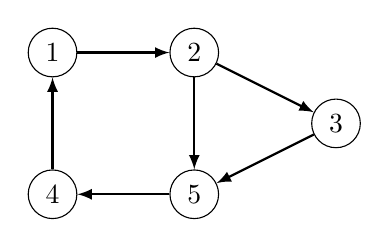
\begin{tikzpicture}[scale=0.9]
\node[draw, circle] (1) at (1,5) {$1$};
\node[draw, circle] (2) at (3,5) {$2$};
\node[draw, circle] (3) at (5,4) {$3$};
\node[draw, circle] (4) at (1,3) {$4$};
\node[draw, circle] (5) at (3,3) {$5$};

\path[draw,thick,->,>=latex] (1) -- (2);
\path[draw,thick,->,>=latex] (2) -- (3);
\path[draw,thick,->,>=latex] (4) -- (1);
\path[draw,thick,->,>=latex] (3) -- (5);
\path[draw,thick,->,>=latex] (2) -- (5);
\path[draw,thick,->,>=latex] (5) -- (4);
\end{tikzpicture}
\end{center}
čvorovi 1, 3 i 4 imaju i ulazni stupanj 1 i izlazni stupanj 1,
čvor 2 ima ulazni stupanj 1 i izlazni stupanj 2,
a čvor 5 ima ulazni stupanj 2 i izlazni stupanj 1.
Dakle, graf sadrži Eulerov put
od čvora 2 do čvora 5:
\begin{center}
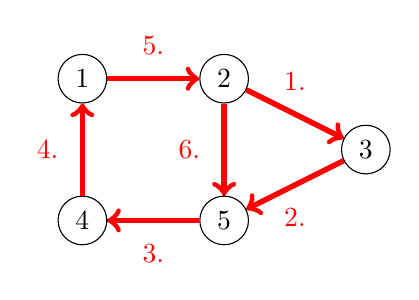
\begin{tikzpicture}[scale=0.9]
\node[draw, circle] (1) at (1,5) {$1$};
\node[draw, circle] (2) at (3,5) {$2$};
\node[draw, circle] (3) at (5,4) {$3$};
\node[draw, circle] (4) at (1,3) {$4$};
\node[draw, circle] (5) at (3,3) {$5$};

\path[draw,thick,-] (1) -- (2);
\path[draw,thick,-] (2) -- (3);
\path[draw,thick,-] (1) -- (4);
\path[draw,thick,-] (3) -- (5);
\path[draw,thick,-] (2) -- (5);
\path[draw,thick,-] (4) -- (5);

\path[draw=red,thick,->,line width=2pt] (2) -- node[font=\small,label={[red]north:1.}] {} (3);
\path[draw=red,thick,->,line width=2pt] (3) -- node[font=\small,label={[red]south:2.}] {} (5);
\path[draw=red,thick,->,line width=2pt] (5) -- node[font=\small,label={[red]south:3.}] {} (4);
\path[draw=red,thick,->,line width=2pt] (4) -- node[font=\small,label={[red]left:4.}] {} (1);
\path[draw=red,thick,->,line width=2pt] (1) -- node[font=\small,label={[red]north:5.}] {} (2);
\path[draw=red,thick,->,line width=2pt] (2) -- node[font=\small,label={[red]left:6.}] {} (5);
\end{tikzpicture}
\end{center}

\subsubsection{Hierholzerov algoritam}

\index{Hierholzerov algoritam}

\key{Hierholzerov algoritam}\footnote{Algoritam je objavljen
1873. godine nakon Hierholzerove smrti \cite{hie73}.} je efikasna
metoda za konstrukciju
Eulerovog ciklusa.
Algoritam se sastoji od nekoliko rundi,
od kojih svaka ciklusu dodaje nove bridove.
Naravno, pretpostavljamo da graf sadrži
Eulerov ciklus; u suprotnom ga Hierholzerov
algoritam ne može pronaći.

Prvo algoritam konstruira ciklus koji sadrži
neke (ne nužno sve) bridove grafa.
Nakon toga algoritam proširuje ciklus
korak po korak dodajući mu podcikluse.
Postupak se nastavlja dok svi bridovi ne budu dodani
u ciklus.

Algoritam proširuje ciklus tako da uvijek pronađe
čvor $x$ koji pripada ciklusu, ali ima
izlazni brid koji nije uključen u ciklus.
Algoritam konstruira novi put iz čvora $x$
koji sadrži samo bridove koji još nisu u ciklusu.
Prije ili kasnije
put će se vratiti u čvor $x$,
čime nastaje podciklus.

Ako graf sadrži samo Eulerov put,
i dalje možemo upotrijebiti Hierholzerov algoritam
kako bismo ga pronašli tako da grafu dodamo dodatni brid
i uklonimo taj brid nakon što je ciklus
konstruiran.
Na primjer, u neusmjerenom grafu
dodatni brid dodajemo između dvaju
čvorova neparnog stupnja.

U nastavku ćemo vidjeti kako Hierholzerov algoritam
konstruira Eulerov ciklus u neusmjerenom grafu.

\subsubsection{Primjer}

\begin{samepage}
Razmotrimo sljedeći graf:
\begin{center}
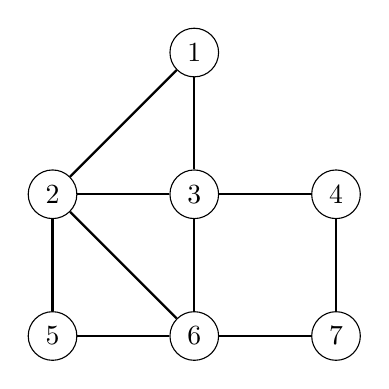
\begin{tikzpicture}[scale=0.9]
\node[draw, circle] (1) at (3,5) {$1$};
\node[draw, circle] (2) at (1,3) {$2$};
\node[draw, circle] (3) at (3,3) {$3$};
\node[draw, circle] (4) at (5,3) {$4$};
\node[draw, circle] (5) at (1,1) {$5$};
\node[draw, circle] (6) at (3,1) {$6$};
\node[draw, circle] (7) at (5,1) {$7$};

\path[draw,thick,-] (1) -- (2);
\path[draw,thick,-] (1) -- (3);
\path[draw,thick,-] (2) -- (3);
\path[draw,thick,-] (2) -- (5);
\path[draw,thick,-] (2) -- (6);
\path[draw,thick,-] (3) -- (4);
\path[draw,thick,-] (3) -- (6);
\path[draw,thick,-] (4) -- (7);
\path[draw,thick,-] (5) -- (6);
\path[draw,thick,-] (6) -- (7);
\end{tikzpicture}
\end{center}
\end{samepage}

\begin{samepage}
Pretpostavimo da algoritam najprije stvara ciklus
koji počinje u čvoru 1.
Mogući ciklus je
$1 \rightarrow 2 \rightarrow 3 \rightarrow 1$:
\begin{center}
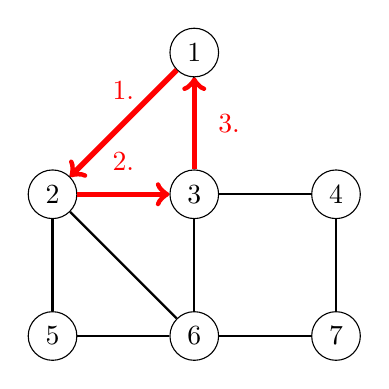
\begin{tikzpicture}[scale=0.9]
\node[draw, circle] (1) at (3,5) {$1$};
\node[draw, circle] (2) at (1,3) {$2$};
\node[draw, circle] (3) at (3,3) {$3$};
\node[draw, circle] (4) at (5,3) {$4$};
\node[draw, circle] (5) at (1,1) {$5$};
\node[draw, circle] (6) at (3,1) {$6$};
\node[draw, circle] (7) at (5,1) {$7$};

\path[draw,thick,-] (1) -- (2);
\path[draw,thick,-] (1) -- (3);
\path[draw,thick,-] (2) -- (3);
\path[draw,thick,-] (2) -- (5);
\path[draw,thick,-] (2) -- (6);
\path[draw,thick,-] (3) -- (4);
\path[draw,thick,-] (3) -- (6);
\path[draw,thick,-] (4) -- (7);
\path[draw,thick,-] (5) -- (6);
\path[draw,thick,-] (6) -- (7);

\path[draw=red,thick,->,line width=2pt] (1) -- node[font=\small,label={[red]north:1.}] {} (2);
\path[draw=red,thick,->,line width=2pt] (2) -- node[font=\small,label={[red]north:2.}] {} (3);
\path[draw=red,thick,->,line width=2pt] (3) -- node[font=\small,label={[red]east:3.}] {} (1);
\end{tikzpicture}
\end{center}
\end{samepage}
Nakon toga algoritam dodaje
podciklus
$2 \rightarrow 5 \rightarrow 6 \rightarrow 2$
ciklusu:
\begin{center}
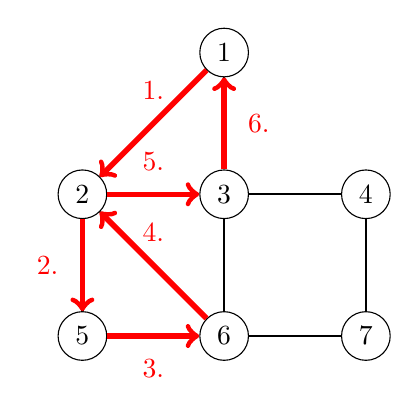
\begin{tikzpicture}[scale=0.9]
\node[draw, circle] (1) at (3,5) {$1$};
\node[draw, circle] (2) at (1,3) {$2$};
\node[draw, circle] (3) at (3,3) {$3$};
\node[draw, circle] (4) at (5,3) {$4$};
\node[draw, circle] (5) at (1,1) {$5$};
\node[draw, circle] (6) at (3,1) {$6$};
\node[draw, circle] (7) at (5,1) {$7$};

\path[draw,thick,-] (1) -- (2);
\path[draw,thick,-] (1) -- (3);
\path[draw,thick,-] (2) -- (3);
\path[draw,thick,-] (2) -- (5);
\path[draw,thick,-] (2) -- (6);
\path[draw,thick,-] (3) -- (4);
\path[draw,thick,-] (3) -- (6);
\path[draw,thick,-] (4) -- (7);
\path[draw,thick,-] (5) -- (6);
\path[draw,thick,-] (6) -- (7);

\path[draw=red,thick,->,line width=2pt] (1) -- node[font=\small,label={[red]north:1.}] {} (2);
\path[draw=red,thick,->,line width=2pt] (2) -- node[font=\small,label={[red]west:2.}] {} (5);
\path[draw=red,thick,->,line width=2pt] (5) -- node[font=\small,label={[red]south:3.}] {} (6);
\path[draw=red,thick,->,line width=2pt] (6) -- node[font=\small,label={[red]north:4.}] {} (2);
\path[draw=red,thick,->,line width=2pt] (2) -- node[font=\small,label={[red]north:5.}] {} (3);
\path[draw=red,thick,->,line width=2pt] (3) -- node[font=\small,label={[red]east:6.}] {} (1);
\end{tikzpicture}
\end{center}
Konačno, algoritam ciklusu dodaje
podciklus
$6 \rightarrow 3 \rightarrow 4 \rightarrow 7 \rightarrow 6$:
\begin{center}
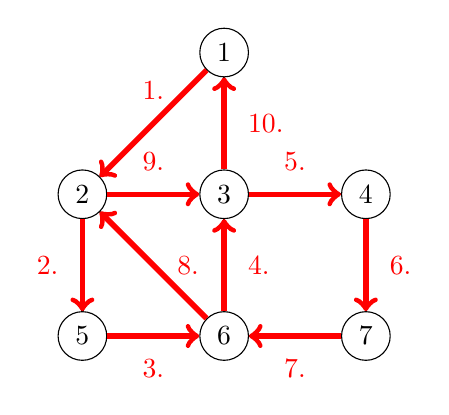
\begin{tikzpicture}[scale=0.9]
\node[draw, circle] (1) at (3,5) {$1$};
\node[draw, circle] (2) at (1,3) {$2$};
\node[draw, circle] (3) at (3,3) {$3$};
\node[draw, circle] (4) at (5,3) {$4$};
\node[draw, circle] (5) at (1,1) {$5$};
\node[draw, circle] (6) at (3,1) {$6$};
\node[draw, circle] (7) at (5,1) {$7$};

\path[draw,thick,-] (1) -- (2);
\path[draw,thick,-] (1) -- (3);
\path[draw,thick,-] (2) -- (3);
\path[draw,thick,-] (2) -- (5);
\path[draw,thick,-] (2) -- (6);
\path[draw,thick,-] (3) -- (4);
\path[draw,thick,-] (3) -- (6);
\path[draw,thick,-] (4) -- (7);
\path[draw,thick,-] (5) -- (6);
\path[draw,thick,-] (6) -- (7);

\path[draw=red,thick,->,line width=2pt] (1) -- node[font=\small,label={[red]north:1.}] {} (2);
\path[draw=red,thick,->,line width=2pt] (2) -- node[font=\small,label={[red]west:2.}] {} (5);
\path[draw=red,thick,->,line width=2pt] (5) -- node[font=\small,label={[red]south:3.}] {} (6);
\path[draw=red,thick,->,line width=2pt] (6) -- node[font=\small,label={[red]east:4.}] {} (3);
\path[draw=red,thick,->,line width=2pt] (3) -- node[font=\small,label={[red]north:5.}] {} (4);
\path[draw=red,thick,->,line width=2pt] (4) -- node[font=\small,label={[red]east:6.}] {} (7);
\path[draw=red,thick,->,line width=2pt] (7) -- node[font=\small,label={[red]south:7.}] {} (6);
\path[draw=red,thick,->,line width=2pt] (6) -- node[font=\small,label={[red]right:8.}] {} (2);
\path[draw=red,thick,->,line width=2pt] (2) -- node[font=\small,label={[red]north:9.}] {} (3);
\path[draw=red,thick,->,line width=2pt] (3) -- node[font=\small,label={[red]east:10.}] {} (1);
\end{tikzpicture}
\end{center}
Sada su svi bridovi uključeni u ciklus,
pa smo uspješno konstruirali Eulerov ciklus.

\section{Hamiltonovi putovi}

\index{Hamiltonov put}

\key{Hamiltonov put}
%\footnote{W. R. Hamilton (1805--1865) bio je irski matematičar.}
je put
koji posjećuje svaki čvor grafa točno jednom.
Na primjer, graf
\begin{center}
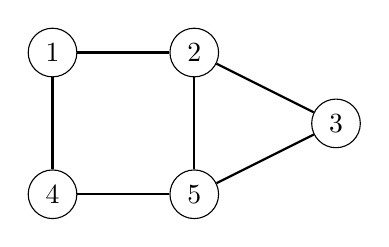
\begin{tikzpicture}[scale=0.9]
\node[draw, circle] (1) at (1,5) {$1$};
\node[draw, circle] (2) at (3,5) {$2$};
\node[draw, circle] (3) at (5,4) {$3$};
\node[draw, circle] (4) at (1,3) {$4$};
\node[draw, circle] (5) at (3,3) {$5$};

\path[draw,thick,-] (1) -- (2);
\path[draw,thick,-] (2) -- (3);
\path[draw,thick,-] (1) -- (4);
\path[draw,thick,-] (3) -- (5);
\path[draw,thick,-] (2) -- (5);
\path[draw,thick,-] (4) -- (5);
\end{tikzpicture}
\end{center}
sadrži Hamiltonov put od čvora 1 do čvora 3:
\begin{center}
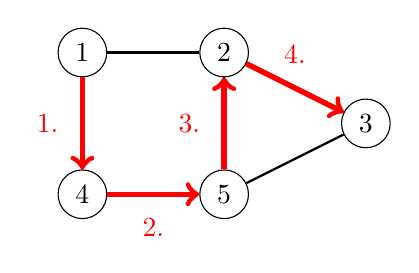
\begin{tikzpicture}[scale=0.9]
\node[draw, circle] (1) at (1,5) {$1$};
\node[draw, circle] (2) at (3,5) {$2$};
\node[draw, circle] (3) at (5,4) {$3$};
\node[draw, circle] (4) at (1,3) {$4$};
\node[draw, circle] (5) at (3,3) {$5$};

\path[draw,thick,-] (1) -- (2);
\path[draw,thick,-] (2) -- (3);
\path[draw,thick,-] (1) -- (4);
\path[draw,thick,-] (3) -- (5);
\path[draw,thick,-] (2) -- (5);
\path[draw,thick,-] (4) -- (5);

\path[draw=red,thick,->,line width=2pt] (1) -- node[font=\small,label={[red]left:1.}] {} (4);
\path[draw=red,thick,->,line width=2pt] (4) -- node[font=\small,label={[red]south:2.}] {} (5);
\path[draw=red,thick,->,line width=2pt] (5) -- node[font=\small,label={[red]left:3.}] {} (2);
\path[draw=red,thick,->,line width=2pt] (2) -- node[font=\small,label={[red]north:4.}] {} (3);
\end{tikzpicture}
\end{center}

\index{Hamiltonov ciklus}

Ako Hamiltonov put počinje i završava u istom čvoru,
naziva se \key{Hamiltonov ciklus}.
Gornji graf ima i Hamiltonov ciklus
koji počinje i završava u čvoru 1:
\begin{center}
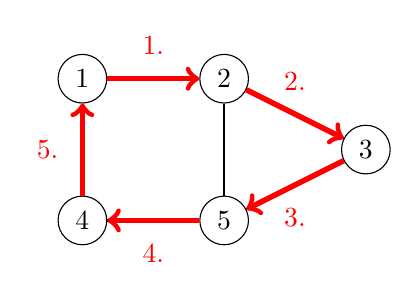
\begin{tikzpicture}[scale=0.9]
\node[draw, circle] (1) at (1,5) {$1$};
\node[draw, circle] (2) at (3,5) {$2$};
\node[draw, circle] (3) at (5,4) {$3$};
\node[draw, circle] (4) at (1,3) {$4$};
\node[draw, circle] (5) at (3,3) {$5$};

\path[draw,thick,-] (1) -- (2);
\path[draw,thick,-] (2) -- (3);
\path[draw,thick,-] (1) -- (4);
\path[draw,thick,-] (3) -- (5);
\path[draw,thick,-] (2) -- (5);
\path[draw,thick,-] (4) -- (5);

\path[draw=red,thick,->,line width=2pt] (1) -- node[font=\small,label={[red]north:1.}] {} (2);
\path[draw=red,thick,->,line width=2pt] (2) -- node[font=\small,label={[red]north:2.}] {} (3);
\path[draw=red,thick,->,line width=2pt] (3) -- node[font=\small,label={[red]south:3.}] {} (5);
\path[draw=red,thick,->,line width=2pt] (5) -- node[font=\small,label={[red]south:4.}] {} (4);
\path[draw=red,thick,->,line width=2pt] (4) -- node[font=\small,label={[red]left:5.}] {} (1);
\end{tikzpicture}
\end{center}

\subsubsection{Postojanje}

Nije poznata nijedna efikasna metoda za provjeru sadrži li graf
Hamiltonov put, a taj je problem NP-težak.
Ipak, u nekim posebnim slučajevima možemo biti sigurni
da graf sadrži Hamiltonov put.

Jednostavno zapažanje jest da ako je graf potpun,
tj. ako postoji brid između svakog para čvorova,
tada sadrži i Hamiltonov put.
Postignuti su i jači rezultati:

\begin{itemize}
\item
\index{Diracov teorem}
\key{Diracov teorem}: %\cite{dir52}
Ako je stupanj svakog čvora barem $n/2$,
graf sadrži Hamiltonov put.
\item
\index{Oreov teorem}
\key{Oreov teorem}: %\cite{ore60}
Ako je suma stupnjeva svakog para nesusjednih čvorova
barem $n$,
graf sadrži Hamiltonov put.
\end{itemize}

Zajedničko svojstvo tih teorema i drugih rezultata jest
da jamče postojanje Hamiltonovog puta
ako graf ima \emph{velik broj} bridova.
To ima smisla jer što graf sadrži više bridova,
to je više mogućnosti za konstrukciju Hamiltonovog puta.

\subsubsection{Konstrukcija}

Budući da ne postoji efikasan način provjere postoji li
Hamiltonov put, jasno je da ne postoji ni metoda
za efikasnu konstrukciju tog puta, jer bismo inače
jednostavno mogli pokušati konstruirati put i vidjeti
postoji li.

Jednostavan način traženja Hamiltonovog puta jest
korištenje algoritma s vraćanjem (backtracking) koji prolazi kroz sve
moguće načine konstrukcije puta.
Vremenska složenost takvog algoritma je barem $O(n!)$,
jer postoji $n!$ različitih načina odabira poretka $n$ čvorova.

Efikasnije rješenje temelji se na dinamičkom programiranju
(vidi poglavlje 10.5).
Ideja je izračunati vrijednosti
funkcije $\texttt{possible}(S,x)$,
gdje je $S$ podskup čvorova, a $x$
jedan od čvorova.
Funkcija govori postoji li Hamiltonov put
koji posjećuje čvorove iz $S$ i završava u čvoru $x$.
To je rješenje moguće implementirati u $O(2^n n^2)$ vremenu.

\section{De Bruijnovi nizovi}

\index{De Bruijnov niz}

\key{De Bruijnov niz}
je znakovni niz koji sadrži
svaki znakovni niz duljine $n$
točno jednom kao podniz znakova, za fiksnu
abecedu od $k$ znakova.
Duljina takvog znakovnog niza je 
$k^n+n-1$ znakova.
Na primjer, kada je $n=3$ i $k=2$,
primjer De Bruijnovog niza je
\[0001011100.\]
Podnizovi znakova tog znakovnog niza su sve
kombinacije triju bitova:
000, 001, 010, 011, 100, 101, 110 i 111.

Pokazuje se da svaki De Bruijnov niz
odgovara Eulerovom putu u grafu.
Ideja je konstruirati graf u kojem
svaki čvor sadrži znakovni niz od $n-1$ znakova,
a svaki brid nizu dodaje jedan znak.
Sljedeći graf odgovara gore opisanoj situaciji:

\begin{center}
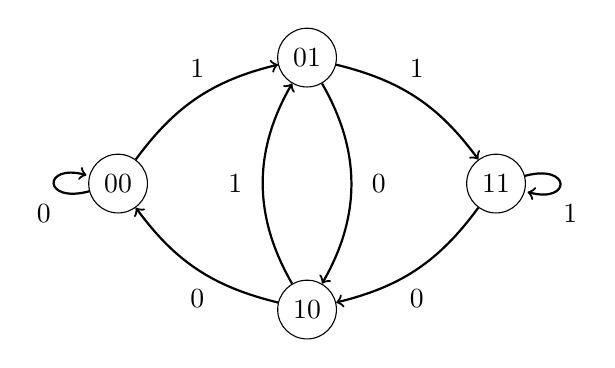
\begin{tikzpicture}[scale=0.8]
\node[draw, circle] (00) at (-3,0) {00};
\node[draw, circle] (11) at (3,0) {11};
\node[draw, circle] (01) at (0,2) {01};
\node[draw, circle] (10) at (0,-2) {10};

\path[draw,thick,->] (00) edge [bend left=20] node[font=\small,label=1] {} (01);
\path[draw,thick,->] (01) edge [bend left=20] node[font=\small,label=1] {} (11);
\path[draw,thick,->] (11) edge [bend left=20] node[font=\small,label=below:0] {} (10);
\path[draw,thick,->] (10) edge [bend left=20] node[font=\small,label=below:0] {} (00);

\path[draw,thick,->] (01) edge [bend left=30] node[font=\small,label=right:0] {} (10);
\path[draw,thick,->] (10) edge [bend left=30] node[font=\small,label=left:1] {} (01);

\path[draw,thick,-] (00) edge [loop left] node[font=\small,label=below:0] {} (00);
\path[draw,thick,-] (11) edge [loop right] node[font=\small,label=below:1] {} (11);
\end{tikzpicture}
\end{center}

Eulerov put u tom grafu odgovara znakovnom nizu
koji sadrži sve znakovne nizove duljine $n$.
Taj znakovni niz sadrži znakove početnog čvora
i sve znakove bridova.
Početni čvor ima $n-1$ znakova,
a na bridovima se nalazi $k^n$ znakova,
pa je duljina znakovnog niza $k^n+n-1$.

\section{Skakačeve ture}

\index{skakačeva tura}

\key{Skakačeva tura} je niz poteza
skakača na šahovskoj ploči dimenzija $n \times n$
prema pravilima šaha takav da skakač
posjeti svako polje točno jednom.
Skakačeva tura naziva se \emph{zatvorenom} turom
ako se skakač na kraju vrati na početno polje, a
inače se naziva \emph{otvorenom} turom.

Na primjer, ovdje je otvorena skakačeva tura na ploči $5 \times 5$:

\begin{center}
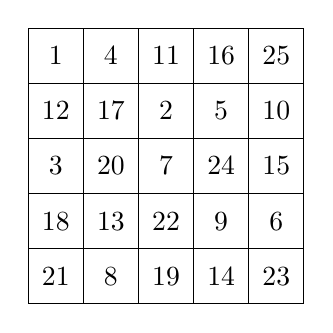
\begin{tikzpicture}[scale=0.7]
\draw (0,0) grid (5,5);
\node at (0.5,4.5) {$1$};
\node at (1.5,4.5) {$4$};
\node at (2.5,4.5) {$11$};
\node at (3.5,4.5) {$16$};
\node at (4.5,4.5) {$25$};
\node at (0.5,3.5) {$12$};
\node at (1.5,3.5) {$17$};
\node at (2.5,3.5) {$2$};
\node at (3.5,3.5) {$5$};
\node at (4.5,3.5) {$10$};
\node at (0.5,2.5) {$3$};
\node at (1.5,2.5) {$20$};
\node at (2.5,2.5) {$7$};
\node at (3.5,2.5) {$24$};
\node at (4.5,2.5) {$15$};
\node at (0.5,1.5) {$18$};
\node at (1.5,1.5) {$13$};
\node at (2.5,1.5) {$22$};
\node at (3.5,1.5) {$9$};
\node at (4.5,1.5) {$6$};
\node at (0.5,0.5) {$21$};
\node at (1.5,0.5) {$8$};
\node at (2.5,0.5) {$19$};
\node at (3.5,0.5) {$14$};
\node at (4.5,0.5) {$23$};
\end{tikzpicture}
\end{center}

Skakačeva tura odgovara Hamiltonovom putu u grafu
čiji čvorovi predstavljaju polja ploče,
a dva su čvora povezana bridom ako se skakač
može premjestiti između tih polja prema pravilima šaha.

Prirodan način konstrukcije skakačeve ture jest korištenje vraćanja (backtracking).
Pretraživanje se može učiniti efikasnijim korištenjem
\emph{heuristika} koje pokušavaju voditi skakača tako da
se potpuna tura brzo pronađe.

\subsubsection{Warnsdorfovo pravilo}

\index{heuristika}
\index{Warnsdorfovo pravilo}

\key{Warnsdorfovo pravilo} je jednostavna i djelotvorna heuristika
za pronalazak skakačeve ture\footnote{Tu je heuristiku predložio
Warnsdorf u svojoj knjizi \cite{war23} 1823. godine. Postoje
i polinomijalni algoritmi za pronalazak skakačevih tura
\cite{par97}, ali su složeniji.}.
Pomoću tog pravila moguće je efikasno konstruirati turu
čak i na velikoj ploči.
Ideja je skakača uvijek pomaknuti tako da završi
na polju na kojem je broj mogućih poteza što
\emph{manji}.

Na primjer, u sljedećoj situaciji postoji pet
mogućih polja na koja se skakač može pomaknuti (polja $a \ldots e$):
\begin{center}
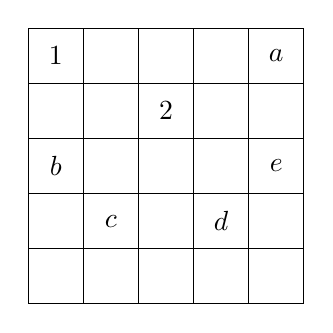
\begin{tikzpicture}[scale=0.7]
\draw (0,0) grid (5,5);
\node at (0.5,4.5) {$1$};
\node at (2.5,3.5) {$2$};
\node at (4.5,4.5) {$a$};
\node at (0.5,2.5) {$b$};
\node at (4.5,2.5) {$e$};
\node at (1.5,1.5) {$c$};
\node at (3.5,1.5) {$d$};
\end{tikzpicture}
\end{center}
U toj situaciji Warnsdorfovo pravilo pomiče skakača na polje $a$,
jer nakon tog izbora postoji samo jedan mogući potez.
Ostali bi izbori pomaknuli skakača na polja na kojima
bi bila dostupna tri poteza.


